% !TeX root = ../main.tex
\section{Results}
\label{sec:results}

% --------------------------------------------------------
\subsection{Sentinel-1 signatures of historical stand disturbances}
\label{sec:s1_signatures}
% --------------------------------------------------------

Historical stand disturbances were expressed as sustained within-stand declines in Sentinel-1 backscatter despite substantial overlap in absolute backscatter states (Fig.~\ref{fig:s1_population_signatures}). Across all observations from the 3,498 balsa polygons, the 5th--95th percentile ranges were $-9.3$ to $-5.0$~dB for VV and $-15.7$ to $-11.5$~dB for VH. Among dated-reference events, median VV changed from $-6.0$~dB before disturbance to $-7.5$~dB during months 0 to $+2$, while VH changed from $-12.5$ to $-14.0$~dB. The pre- and post-event distributions nevertheless remained broadly overlapping, indicating that absolute backscatter alone did not provide a stable threshold for separating stand states (Fig.~\ref{fig:s1_population_signatures}a).

\begin{figure*}[pos=!htbp]
    \centering
    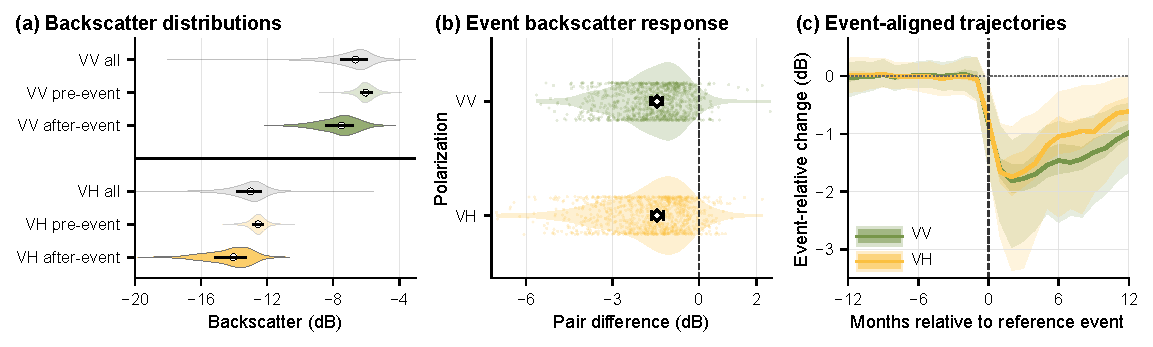
\includegraphics[width=\linewidth]{figures/fig05_population_s1_signatures.pdf}
    \caption{Sentinel-1 signatures of balsa stand disturbances.
    (a) Absolute VV and VH distributions across all observations from the 3,498 polygons and within the pre-event ($-12$ to $-3$ months) and event/post-event (0 to $+2$ months) periods.
    (b) Paired event/post-minus-pre changes for 1,018 reference events; diamonds show medians and bars show 95\% complete-spatial-block bootstrap confidence intervals.
    (c) Event-aligned deviations from the pre-event background; dark and light ribbons show interquartile ranges and pointwise 95\% block-bootstrap confidence intervals, respectively.}
    \label{fig:s1_population_signatures}
\end{figure*}

Within-event changes were considerably more consistent than the absolute backscatter values. Across 1,018 reference events, median event/post-minus-pre change was $-1.46$~dB for VV (95\% spatial-block bootstrap CI, $-1.66$ to $-1.26$~dB) and $-1.45$~dB for VH ($-1.64$ to $-1.23$~dB), with negative changes in 96.4\% and 94.1\% of events, respectively (Fig.~\ref{fig:s1_population_signatures}b). Event-aligned median departures reached approximately $-1.8$~dB by month $+2$ and remained negative at month $+12$ ($-1.0$~dB for VV and $-0.6$~dB for VH); pointwise 95\% block-bootstrap intervals remained below zero throughout this period (Fig.~\ref{fig:s1_population_signatures}c). These results show that disturbance was more consistently expressed as a relative departure from the recent stand background than as an absolute backscatter state.

The representative stand showed the same temporal pattern (Fig.~\ref{fig:timeseries_signature}). The March 2024 reference disturbance coincided with coherent VV and VH declines and an optical transition from dense canopy to exposed ground, while earlier events in April 2019 and February 2022 illustrated repeated disturbance--recovery dynamics within the same stand. Similar absolute backscatter levels occurred during different stages of recovery and disturbance, further illustrating the value of interpreting change relative to the stand's recent temporal context.

% ---------------------------------------------------------------
\subsection{Sensitivity to stand representation, window geometry, and polarization}
\label{sec:representation_configuration}
% ---------------------------------------------------------------

Detection performance was generally stable across reasonable choices of stand representation, window geometry, and polarization, with no alternative providing a clear F1 improvement over the retained configuration (Fig.~\ref{fig:stand_representation_sensitivity}).

\begin{figure*}[pos=!htbp]
    \centering
    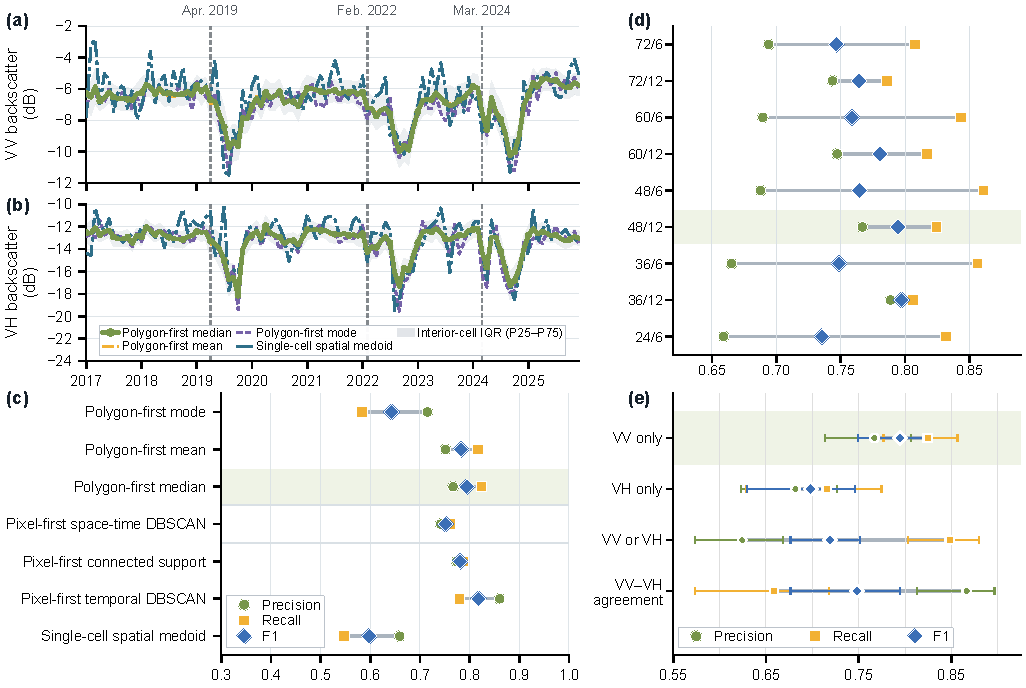
\includegraphics[width=\linewidth]{figures/fig07_representation_configuration.pdf}
    \caption{Sensitivity of Windowed CUSUM to stand representation, window geometry, and polarization.
    (a,b) Illustrative monthly VV and VH stand trajectories with within-polygon cell interquartile ranges and reference-event months.
    (c--e) Event-level precision, recall, and F1 across stand representations, window configurations, and polarization strategies.
    Connected support used the spatially selected threshold $r=0.20$; whiskers show 95\% spatial-block bootstrap confidence intervals, and highlighting indicates the retained configurations.}
    \label{fig:stand_representation_sensitivity}
\end{figure*}


Under the fixed 48-month window, 12-month displacement, and $p_{\mathrm{perm}}\leq0.025$ threshold, the Polygon-first median achieved precision 0.767, recall 0.824, and F1 0.795. The highest alternative point estimate was obtained by Pixel-first temporal DBSCAN (F1 = 0.818), but its paired F1 advantage was uncertain ($+0.024$, 95\% CI: $-0.005$ to 0.049). Connected support with the spatially selected $r=0.20$ achieved precision 0.774, recall 0.788, and F1 0.781, differing from the median by $-0.014$ (95\% CI: $-0.034$ to 0.007). The Polygon-first median was therefore retained because it provided a direct stand-level trajectory, high recall, and no additional support or clustering parameters.

Window geometry had similarly limited influence near the retained configuration. The highest fixed F1 was 0.797 for 36/12, only $+0.003$ above 48/12 (95\% CI: $-0.013$ to 0.019). Although 36/12 was selected in all five outer folds, its nested spatial out-of-fold performance remained essentially equivalent to the prospectively locked 48/12 configuration. The 48/12 geometry was therefore retained.

VV-only produced the highest F1 among the evaluated polarization strategies (precision 0.767, recall 0.824, F1 0.795). Accepting detections from either polarization increased recall at the expense of precision, whereas requiring VV--VH agreement increased precision but reduced recall. Neither strategy improved F1, and VV-only was retained for the final disturbance-history reconstruction.


% -----------------------------------------------------------
\subsection{Component attribution of Windowed CUSUM}
\label{sec:representation_component_ablation}
% -----------------------------------------------------------

Component analysis showed that local-reference windowing was the main source of recurrent-event sensitivity, while central-interval admission and permutation calibration progressively recovered precision (Table~\ref{tab:component_ablation}). Adding local-reference windows increased recall from 0.349 to 0.878 and F1 by $+0.137$ (95\% CI: 0.075--0.198), although precision decreased to 0.493. Central-interval admission increased precision to 0.684 and produced a further F1 gain of $+0.127$ (0.103--0.146). The negative-shift constraint had negligible incremental effect, whereas permutation-based calibration increased precision from 0.687 to 0.767 and F1 by $+0.036$ (0.022--0.049), yielding the complete detector F1 of 0.795.

\begin{table*}[pos=!htbp]
    \centering
    \small
    \caption{Progressive component attribution under the fixed 48/12 configuration. $\Delta F1$ compares each cumulative configuration with its predecessor; intervals are paired 95\% spatial-block bootstrap confidence intervals.}
    \label{tab:component_ablation}

    \begin{tabular}{lrrrrc}
        \toprule
        Cumulative configuration &
        Detections &
        Precision &
        Recall &
        F1 &
        Incremental $\Delta F1$ [95\% CI] \\
        \midrule
        Global CUSUM
        & 447
        & 0.852
        & 0.349
        & 0.495
        & -- \\

        + Local-reference windows
        & 1,948
        & 0.493
        & 0.878
        & 0.631
        & $+0.137$ [0.075, 0.198] \\

        + Central decision interval
        & 1,362
        & 0.684
        & 0.852
        & 0.758
        & $+0.127$ [0.103, 0.146] \\

        + Negative-shift constraint
        & 1,350
        & 0.687
        & 0.848
        & 0.759
        & $+0.000$ [$-0.003$, 0.003] \\

        + Permutation-based calibration
        & 1,175
        & 0.767
        & 0.824
        & \textbf{0.795}
        & $+0.036$ [0.022, 0.049] \\
        \bottomrule
    \end{tabular}
\end{table*}

Controlled-removal analysis supported the same ordering. Removing local-reference windowing reduced F1 by 0.327 (95\% CI: 0.280--0.370), compared with reductions of 0.038 for the central decision interval and 0.036 for permutation calibration; removing the negative-shift constraint again had negligible effect. Together, the two analyses indicate that recurrent-event sensitivity was driven primarily by repeated local-reference renewal, whereas central admission and local statistical calibration controlled the precision lost when additional candidate events became detectable. Because the Global CUSUM baseline can nominate only one candidate per trajectory, this contrast isolates component contributions within the ablation framework and is not a substitute for comparison with recurrent benchmark detectors.



% -----------------------------------------------------------
\subsection{Benchmark performance and statistical robustness}
\label{sec:benchmark_null_sensitivity}
% -----------------------------------------------------------

Under five-fold spatial out-of-fold evaluation, Windowed CUSUM achieved precision 0.789, recall 0.806, F1 0.797, and matched-event MAE 0.776 months (Table~\ref{tab:benchmark_comparison}). The highest benchmark F1 was 0.680 for CCDC, followed by 0.675 for decrease-filtered ReCuSum. Primary F1 differences were $+0.117$ against CCDC (97.5\% CI: 0.085--0.172) and $+0.454$ against monthly CuSum NRT (97.5\% CI: 0.412--0.491). ReCuSum attained similar precision to Windowed CUSUM (0.787 versus 0.789) but substantially lower recall (0.591 versus 0.806); the paired F1 difference was $+0.122$ (95\% CI: 0.094--0.149). Thus, the advantage over this recurrent detector arose primarily from improved event recall.

Exploratory CCDC expansion yielded F1 0.669 (change $-0.011$, 95\% CI: $-0.023$ to 0.005), without evidence of improvement. On 626 shared reference events, Windowed CUSUM had higher MAE than original CCDC (difference 0.101 months, 95\% CI: 0.014--0.205). The Windowed CUSUM advantage concerned detection balance, not uniformly higher recall or lower dating error.

\begin{table}[pos=!htbp]
    \centering
    \small
    \caption{Five-fold spatial out-of-fold benchmark using Polygon-first median VV trajectories and $\pm2$-month event matching. CCDC uses the original search; MAE includes matched events only.
    }
    \label{tab:benchmark_comparison}

    \begin{tabular}{lrrrr}
        \toprule
        Evaluated implementation & Precision & Recall & F1 & MAE (months) \\
        \midrule
        \textbf{Windowed CUSUM}
        & 0.789 & 0.806 & \textbf{0.797} & 0.776 \\

        CCDC 
        & 0.750 & 0.622 & 0.680 & 0.626 \\

        ReCuSum, decrease-filtered
        & 0.787 & 0.591 & 0.675 & 0.752 \\

        CuSum NRT, decrease-filtered
        & 0.414 & 0.844 & 0.556 & 0.875 \\

        BOCD prototype, decrease-filtered
        & 0.740 & 0.343 & 0.469 & 0.747 \\

        ReCuSum, raw
        & 0.419 & 0.513 & 0.461 & 0.743 \\

        Maximum monthly decline
        & 0.335 & 0.572 & 0.422 & 0.755 \\

        CuSum NRT, monthly adaptation
        & 0.222 & 0.754 & 0.344 & 0.898 \\

        Classical lower CUSUM
        & 0.171 & 0.290 & 0.215 & 1.498 \\
        \bottomrule
    \end{tabular}
\end{table}

The recall advantage over decrease-filtered ReCuSum was most pronounced in polygons with multiple recorded disturbances. For polygons containing one, two, and at least three reference events, Windowed CUSUM achieved recalls of 0.891, 0.813, and 0.794, compared with 0.764, 0.624, and 0.553 for ReCuSum. In the at-least-three-event group, the paired recall difference reached $+0.240$ (95\% CI: 0.179--0.289), consistent with the intended role of local-reference renewal in recurrent-event detection. These strata describe recorded reference-event multiplicity and are not assumed to represent complete disturbance histories.

Temporal-null formulation primarily shifted the precision--recall operating point. Under the fixed 48/12 configuration, finite-sample independent-value permutation yielded F1 0.795, compared with 0.791 for the archived empirical-rank implementation. A three-month calendar-block permutation increased precision to 0.828 but reduced recall to 0.676 and F1 to 0.745 ($\Delta F1=-0.050$, 95\% CI: $-0.084$ to $-0.028$). Six-month blocks further reduced recall to 0.339, while 12-month blocks admitted no events at the common threshold. Moving-block-bootstrap nulls yielded F1 values of 0.667--0.725, and the track-wise maximum-statistic null yielded 0.365. Monte Carlo seed variation was negligible relative to differences among null formulations. The independent-value permutation therefore provided the highest F1 under the common threshold, although this comparison demonstrates sensitivity to null assumptions rather than establishing its statistical calibration as uniquely correct.


% 需要多少 post-event evidence 才能稳定检测？冻结后的方法在真实 incomplete terminal record 上能否运行？
% -----------------------------------------------------------
\subsection{Temporal truncation and prospective performance}
\label{sec:temporal_prospective_results}
% -----------------------------------------------------------

Temporal truncation showed that detection sensitivity increased as post-disturbance evidence accumulated. Among the 1,065 reference events evaluable at every horizon, recall increased from 0.202 using observations available only through the reference month to 0.613 after three months, 0.790 after six months, and 0.849 after 12 months. Event timing was comparatively stable once a detection had been established: of the 841 events detected by the six-month horizon, 814 (96.8\%) were assigned a month within $\pm2$ months of their corresponding 12-month estimate. Thus, limited post-event support primarily constrained whether an event was detected, rather than the stability of its estimated timing once sufficient evidence had accumulated.

A prospective replay of the locked detector using observations available through June 2026 produced 139 provisional disturbance candidates. Manual review was conducted for 95 sampled candidate polygons. After accounting for the prespecified sampling fractions, 57.5\% of candidates were estimated to represent confirmed disturbances (95\% spatial-block bootstrap CI: 0.287--0.812), increasing to 64.0\% (95\% CI: 0.393--0.846) when probable disturbances were included. Because validation was conditioned on detector-generated candidates, these estimates characterize candidate precision and prospective behaviour, but do not quantify missed disturbances or population recall.

% -----------------------------------------------------------------------
% -----------------------------------------------------------------------
\subsection{Recurrent disturbance histories and rotation-relevant intervals}
\label{sec:rotation_dynamics}
% -----------------------------------------------------------------------

Application of the locked VV-only Windowed CUSUM to the 3,498 validated balsa polygons identified 6,658 disturbance events during 2017--2025 (Fig.~\ref{fig:national_recurrence_patterns}). Event recurrence showed marked spatial heterogeneity, and annual detections ranged from 308 in 2023 to 1,026 in 2022. 
% Across the inventory, 82.9\% of polygons contained one to three detected events, whereas 349 contained none.

Among the 2,194 polygons with at least two detections, consecutive events defined 3,509 inter-disturbance intervals. The median interval was 36 months (IQR: 22--46 months; 95\% spatial-block bootstrap CI: 35--38 months), and 53.0\% of intervals fell between 24 and 47 months (Fig.~\ref{fig:national_recurrence_patterns}d). Short intervals were also common, with 20.4\% shorter than 12 months, indicating that successive detections cannot all be interpreted as complete plantation rotations.

Cross-polarization analysis tested whether the approximately three-year recurrence was specific to the VV-derived event sequence. Requiring both bounding VV events to have a one-to-one VH match within $\pm2$ months retained 1,385 intervals from 1,081 polygons, representing 39.5\% of all VV intervals (Fig.~\ref{fig:polarization_interval_sensitivity}). Their median was 40 months (IQR: 34--48 months; 95\% CI: 38--41 months), four months longer than the full VV estimate (paired 95\% CI: $+2$ to $+5$ months). VH support was less frequent for short intervals, indicating preferential retention of longer intervals rather than an unbiased correction of the VV distribution. Nevertheless, the dominant approximately three-year recurrence remained evident under cross-polarization support.

These intervals describe recurrent stand turnover observed within the Sentinel-1 record rather than independently verified planting-to-harvest cycles. The 36-month median is therefore interpreted as a rotation-relevant recurrence timescale, while individual disturbance events and short intervals require additional evidence before attribution to harvesting or complete biological rotations.

\begin{figure*}[pos=!htbp]
    \centering
    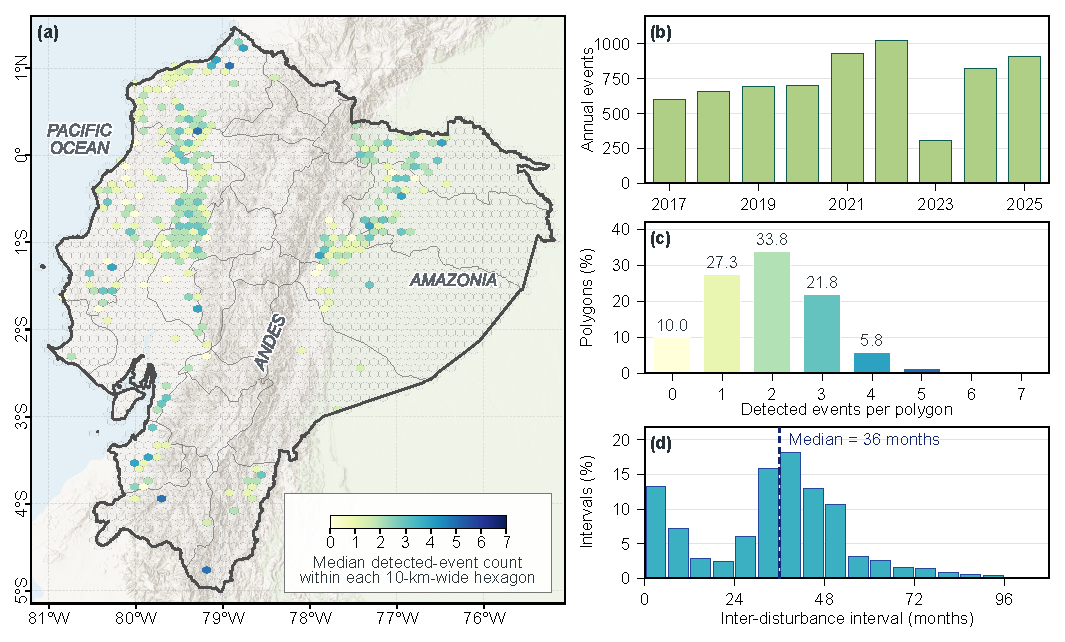
\includegraphics[width=\linewidth]{figures/fig01_national_recurrence.pdf}

    \caption{Reconstructed recurrent disturbances across the Ecuadorian balsa inventory.
    (a) Median detected-event count within fixed 10-km-wide hexagons.
    (b) Annual counts of the 6,658 detected events during 2017--2025.
    (c) Event-count distribution.
    (d) Distribution of 3,509 consecutive inter-disturbance intervals.}

    \label{fig:national_recurrence_patterns}
\end{figure*}

\begin{figure*}[pos=!htbp]
    \centering
    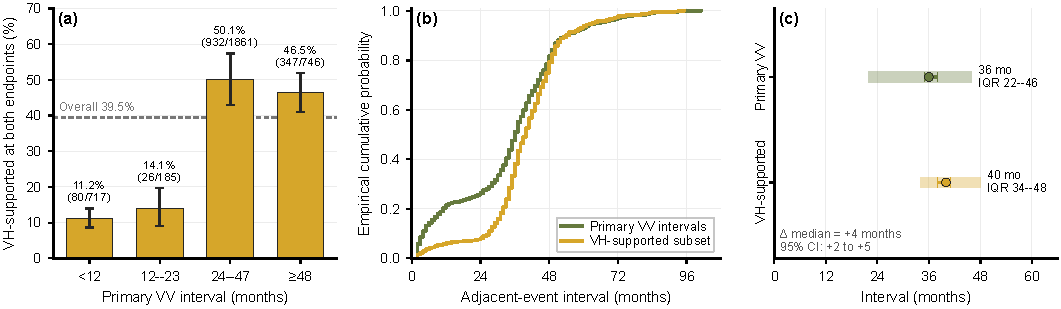
\includegraphics[width=\linewidth]{figures/fig08_polarization_intervals.pdf}

    \caption{Cross-polarization sensitivity of observed inter-disturbance intervals.
    (a) Fraction of VV-defined intervals for which both bounding events had corresponding VH detections within $\pm2$ months.
    (b) Empirical cumulative distributions of all VV intervals ($n=3{,}509$) and the VH-supported subset ($n=1{,}385$).
    (c) Median and interquartile interval estimates with 95\% spatial-block bootstrap confidence intervals.}

    \label{fig:polarization_interval_sensitivity}
\end{figure*}
